\documentclass[11pt]{report}

%-------------PACOTES-----------------%
\usepackage[latin1,utf8]{inputenc}
\usepackage[portuguese]{babel}
\usepackage[nottoc,notlot,notlof]{tocbibind}
\usepackage{graphicx}
\usepackage{float}
\usepackage{caption}
\usepackage{subcaption}
\usepackage{booktabs}
\usepackage{colortbl}
\usepackage{titlepic}
\usepackage{amsmath}
\usepackage{amssymb}
%-------------------------------------%

\begin{document}

%-------------CAPA--------------------%
\titlepic{
\includegraphics[scale=0.5]{logoCiencias}}
\title{Dinâmica de Rotação}
\author{Ana Patrícia 52871\\
		Ernesto González 52857\\
		Gonçalo Jesus 52874\\
		Tiago Pereira 53107}
\date{Física Experimental I\\
	  Faculdade de Ciências - Universidade de Lisboa\\
	  Ano Letivo 2018/2019}
\maketitle
%-------------------------------------%
%-------------ÍNDICE------------------%
\tableofcontents
%-------------------------------------%
%-------------RESUMO------------------%
\chapter{Resumo}
Historiadores e tecnologistas apontam que a roda foi a maior invenção da Humanidade \cite{Bulliet:2016} com diversas aplicações nas engenharias e ciências. Uma roda descreve um movimento rotacional à volta do seu eixo central (ou de rotação). Neste trabalho propômos estudar o movimento de rotação de um corpo rígido, focando a nossa atenção em rotação uni-axial sem translação. Para estes efeitos, escolheu-se uma barra metálica com duas massas cilíndricas de posição ajustável simetricamente dispostas em relação ao centro geométrico da barra. Fixamos a barra em eixo solidário com um disco dividido em sectores alternadamente transparentes e opacos. Enrolado à volta do eixo de rotação está um fio ligado a um peso suspenso por uma roldana (ver Figura \ref{fig:figura1}).

\begin{figure} [h]
\center
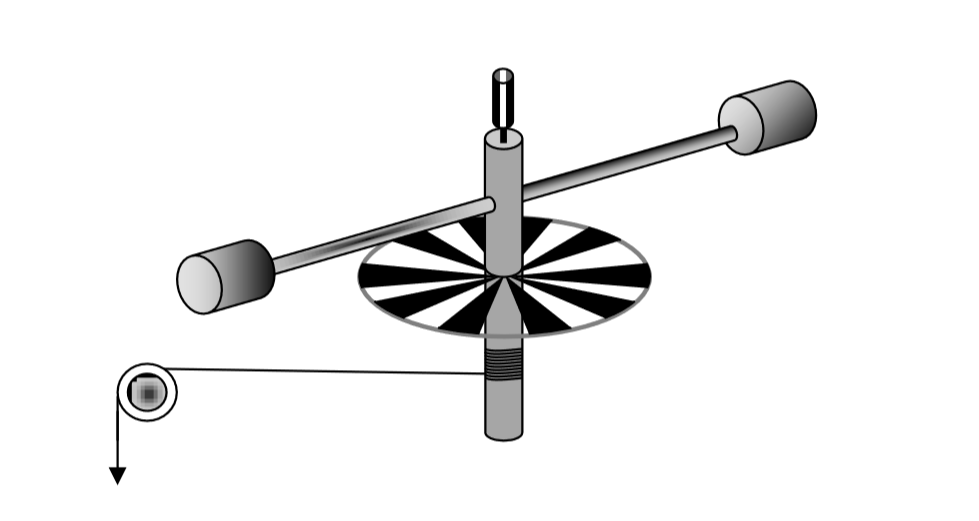
\includegraphics[scale=0.30]{aparelho}
\caption{Esquema do sistema de rotação.\label{fig:figura1}}
\end{figure}

\newpage 
Uma vez que o disco roda juntamente com a barra, é-nos permitida a medição e cálculo das variáveis rotacionais\footnote{\textit{Elapsed time}, período, velocidade angular e aceleração angular.} com uma foto-porta e o {\it DataStudio}\footnote{Software para tratamento de dados.}.
Inicialmente, enquanto o peso suspenso cai, o fio desenrola-se do eixo de rotação, obrigando o sistema a rodar com uma aceleração angular cada vez maior (ver primeiros 10 segundos da Figura \ref{fig:figura2}). Após a queda do peso, com o fio já solto e o sistema livre de forçamento, vemos como a barra roda cada vez mais devagar, eventualmente parando (ver Figura \ref{fig:figura2} após os primeiros 10 segundos).

\begin{figure} [h]
\center
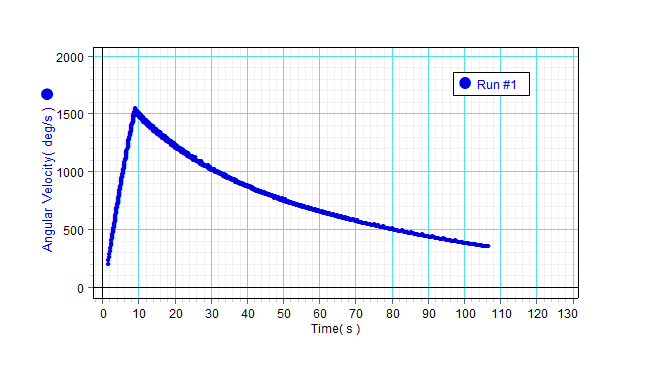
\includegraphics[scale=0.7]{variationOfSpeed}
\caption{Velocidade angular por unidade de tempo. \label{fig:figura2}}
\end{figure}

Atendendo a $I=\sum_im_iR_i^2$ e $M=I\alpha $ vemos que se mudar-mos a distância das massas obtemos momentos de inércia (consequentemente acelerações angulares) diferentes. Seguindo este raciocínio estudamos o movimento do sistema para três distâncias $d$ das massas ao centro de rotação e um caso sem massas (ver Figura\ref{fig:figura3}).

\begin{figure} [h]
\center
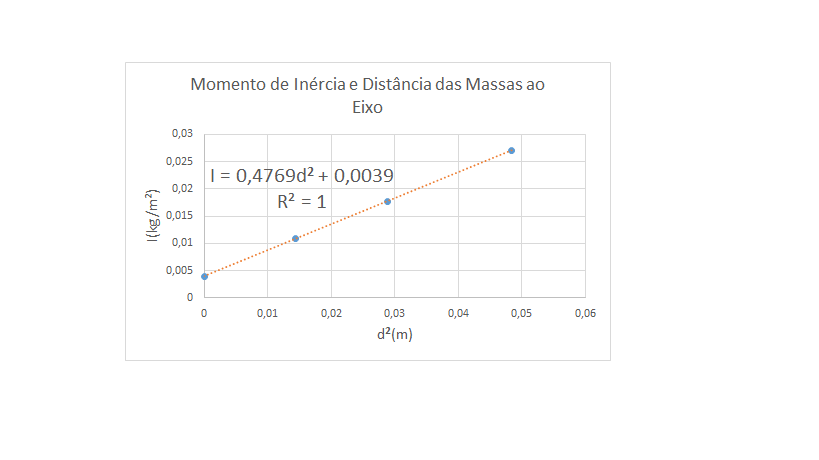
\includegraphics[scale=0.7]{inerciaEDistancia}
\caption{Momento de inércia e distância das massas ao eixo de rotação (d=0 indica ausência das massas cilíndricas). \label{fig:figura3}}
\end{figure}
Vê-mos que a relação entre o momento de inércia do sistema e a o quadrado das distâncias das massas ao centro é linear. A interpretação física das grandezas em jogo permite-nos ainda concluir que a ordenada na origem é o momento de inércia da barra cilíndrica (sem massas adicionais).

%-------------------------------------%
%-------------INTRODUÇÃO--------------%
\chapter{Introdução}
O que têm em comum uma roda gigante, um pião e uma bailarina a executar o \textit{sur le cou-de-pied}\footnote{Pirueta que começa com um pé descansando entre o tornozelo e a base dos gêmeos. Esse pé é elevado para voltar para dentro em direção à perna de apoio para fazer o giro.}? Todos descrevem movimentos de rotação.
Neste trabalho propômos estudar um movimento de rotação de um corpo rígido num referencial fixo. Pretendemos verificar a relação entre o momento de inércia e a aceleração angular, estudar e justificar os diferentes tipos de movimento que o sistema apresenta, caracterizar a aceleração angular do movimento inicial, a aceleração angular média das forças de atrito, a aceleração angular associada ao momento aplicado pela força de tensão do fio em que a massa \textit{m} \footnote{Massa suspensa pelo fio ligado ao eixo de rotação do corpo rígido, que ao cair desencadeia uma aceleração angular crescente no corpo, devido à tensão do fio.} está suspensa, o tipo de movimento da massa \textit{m}, que desce na vertical, a aceleração linear correspondente e a tensão no fio enquanto a massa desce, e finalmente, o momento aplicado pela força de tensão.
Com os valores obtidos, determinamos, em cada caso, o momento de inércia do sistema caracterizado pela incerteza respetiva, bem como a sua dependência com a distância das massas móveis ao centro de rotação.
%-------------------------------------%
%---------FUNDAMENTAÇÃO TEÓRICA-------%
\chapter{Fundamentação Teórica}
O movimento de rotação de um corpo em relação a um ponto O é caracterizado pelo momento angular $\overrightarrow{L}$. Num corpo rígido, constituído por um conjunto de partículas, cada uma com momento angular $\overrightarrow{\ell_i}$ temos $\overrightarrow{L}=\sum_i \overrightarrow{\ell_i}$.
Em qualquer momento do movimento temos $$\frac{d\overrightarrow{\ell}}{dt}= \overrightarrow{r} \times \overrightarrow{F} = \overrightarrow{M}. $$
A variação no tempo do momento angular é igual ao momento (torque) da força aplicada \cite{Cruz}.
Da Geometria, sabemos que $\theta$ é dado por $$\theta = \frac{s}{r} \quad(medida\; em\; radianos). $$
A velocidade angular (instantânea) $\omega$ é $$\omega = \lim_{\Delta t \to 0} \frac{\Delta \theta}{\Delta t}= \frac{d \theta}{dt} $$
e, por sua vez, a aceleração angular (instantânea) consiste em 
$$\alpha = \lim_{\Delta t \to 0} \frac{\Delta \omega}{\Delta t}= \frac{d \omega}{dt}. $$
Associando as grandezas do movimento circular com as do movimento rotacional\footnote{Uma partícula que descreve um movimento circular em volta de um ponto O consiste, em realidade, num sistema rotacional.} ficamos com $$\frac{d\overrightarrow{\ell}}{dt}=I\frac{d\overrightarrow{\omega}}{dt} \iff \overrightarrow{M}=I\overrightarrow{\alpha}.$$\\
O \textit{Teorema dos eixos paralelos} diz que o momento de inércia de um corpo em relação a um eixo de rotação  que passa pelo seu centro de massa, $I_{CM}$ e o seu momento de inércia relativamente a um eixo paralelo ao primeiro, $I_p$ estão relacionados por $$I_p=I_{CM}+md^2$$ onde $d$ é a distância entre os eixos de rotação paralelos e $m$ a massa do sólido\cite{Cruz}.
%-------------------------------------%
%---------MÉTODO E EQUIPAMENTO--------%
\chapter{Método e Equipamento}
O equipamento utilizado na experiência foi:
\begin{itemize}
\item Barra com duas massas cilíndricas de posição ajustável, fixa em eixo solidário com \textit{chopper}\footnote{Disco dividido em sectores alternadamente transparentes e opacos.} que é apoiada num eixo fixo;
\item Massa calibrada;
\item Prato para massas, com fio terminado por fita de velcro; 
\item Roldana;
\item Interface com foto-porta e o programa \textit{DataStudio}.
\end{itemize}

\begin{figure} [h]
\center
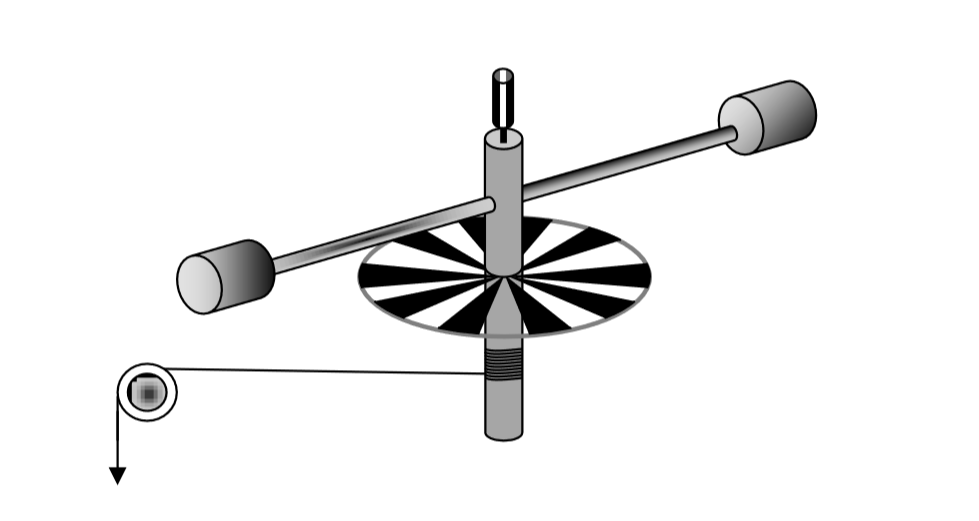
\includegraphics[scale=0.35]{aparelho}
\caption{Esquema do sistema de rotação.\label{fig:figura4}}
\end{figure}

Prendeu-se a barra cilíndrica no eixo de rotação e, por sua vez, as massas cilíndricas a uma distância \textit{d} do centro de rotação. Enrolou-se o fio com a massa ligada à volta do eixo de rotação. Suspendeu-se a massa e deixou-se cair, observando de imediato como, à medida que o fio se ia desenrolando, a barra (consequentemente o disco) rodavam cada vez mais rápido. Entretando, a foto-porta registava o tempo decorrido entre cada interrupção do seu feixe de luz, pelas secções opacas do disco. Com estes tempos, e sabendo o arco de cada secção, o \textit{DataStudio} apresenta-nos o \textit{elapsed-time}, a velocidade angular e aceleração angular.

Repetimos este procedimento três vezes para cada disposição das massas cilíndricas.
Posicionamos as massas cilíndricas a distâncias de $0.12\pm0.05 m$, $0.17\pm0.05 m$, $0.22\pm0.05 m$ e 0$m$ \footnote{A distância ser 0 representa a ausência das massas.}. 
%-------------------------------------%
%-------------RESULTADOS--------------%
\chapter{Resultados}

Com todas as considerações feitas e o planeamento definido, avançamos para a experiência.
O primeiro passo foi determinar a natureza\footnote{Mínima divisão da escala.} e incerteza associada ao equipamento relevante para a experiência (ver Tabela \ref{tabela:5.1}).

\begin{table}[h]
  \centering
    \begin{tabular}{|p{40mm}|p{4.215em}|p{4.215em}|}
    \toprule
    \multicolumn{1}{|r|}{} & \cellcolor[rgb]{ 0,  .69,  .941}\textbf{Natureza} & \cellcolor[rgb]{ 0,  .69,  .941}\textbf{Incerteza} \\
    \midrule
    \rowcolor[rgb]{ 1,  .753,  0} \textbf{Balança Digital} & \cellcolor[rgb]{ 1,  1,  1}0.01g & \cellcolor[rgb]{ 1,  1,  1}0.01g \\
    \midrule
    \rowcolor[rgb]{ 1,  .753,  0} \textbf{Suporte Graduado} & \cellcolor[rgb]{ 1,  1,  1}0.1cm & \cellcolor[rgb]{ 1,  1,  1}0.05cm \\
    \midrule
    \rowcolor[rgb]{ 1,  .753,  0} \textbf{Craveira} & \cellcolor[rgb]{ 1,  1,  1}0.02mm & \cellcolor[rgb]{ 1,  1,  1}0.02mm \\
    \midrule
    \rowcolor[rgb]{ 1,  .753,  0} \textbf{Palmer} & \cellcolor[rgb]{ 1,  1,  1}0.01mm & \cellcolor[rgb]{ 1,  1,  1}0.005mm \\
    \bottomrule
    \end{tabular}%
  \label{tab:addlabel}%
    \caption{Natureza e incerteza do equipamento usado. \label{tabela:5.1}}
\end{table}%

Tendo em conta as incertezas, seguimos para a medição das dimensões de massas e volumes relevantes para a experiência (ver Tabela \ref{tabela:5.2}).
% Table generated by Excel2LaTeX from sheet 'Dados'
\begin{table}[htbp]
  \centering
    \begin{tabular}{|p{50mm}|p{45mm}|}
    \toprule
    \multicolumn{1}{|r|}{\textbf{Dimensões}} & \cellcolor[rgb]{ 0,  .69,  .941}\textbf{Valor} \\
    \midrule
    \rowcolor[rgb]{ 1,  .753,  0} \textbf{Massa do prato} & \cellcolor[rgb]{ 1,  1,  1}$2.14\times 10^{-1} kg\pm 0.005\%$ \\
    \midrule
    \rowcolor[rgb]{ 1,  .753,  0} \textbf{Massa cilíndrica I} & \cellcolor[rgb]{ 1,  1,  1}$2.39 \times 10^{-1}kg \pm 0.004\%$ \\
    \midrule
    \rowcolor[rgb]{ 1,  .753,  0} \textbf{Massa cilíndrica II} & \cellcolor[rgb]{ 1,  1,  1}$2.38 \times 10^{-1}kg \pm 0.004\%$ \\
    \midrule
    \rowcolor[rgb]{ 1,  .753,  0} \textbf{Massa da barra} & \cellcolor[rgb]{ 1,  1,  1}$1.31 \times 10^{-1}kg \pm 0.008\%$ \\
     \midrule
      \rowcolor[rgb]{ 1,  .753,  0} \textbf{Massa suspensa} & \cellcolor[rgb]{ 1,  1,  1}$209.50 \times 10^{-3}kg \pm 0.004\%$ \\
     \midrule
    \rowcolor[rgb]{ 1,  .753,  0} \textbf{Raio do torno\footnote{Cilindro vertical onde está enrolado o fio; eixo de rotação.}} & \cellcolor[rgb]{ 1,  1,  1}$7.75 \times 10^{-3}m \pm 6.45\%$ \\
    \bottomrule
    \end{tabular}%
  \label{tab:addlabel}%
    \caption{Dimensões relevantes das componentes do sistema. \label{tabela:5.2}}
\end{table}%

\newpage
Posteriormente, passamos à relização da esperiência \textit{per se} e obtivemos os seguintes resultados. Nos gráficos e tabelas seguintes apresentamos os dados recolhidos (e analizados com o \textit{DataStudio}).

\begin{figure} [H]
\center
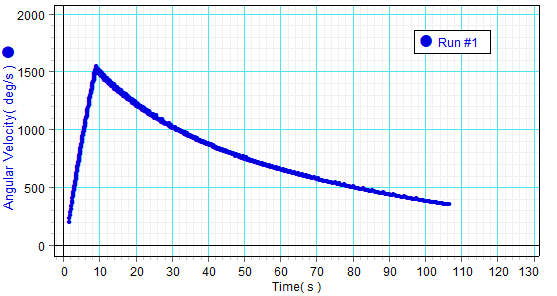
\includegraphics[scale=0.8]{velAngulard1}
\caption{Velocidade angular em função do tempo para $d=0.12\pm0.05 m $. \label{figura:5.1}}
\end{figure}

\begin{figure} [H]
\center
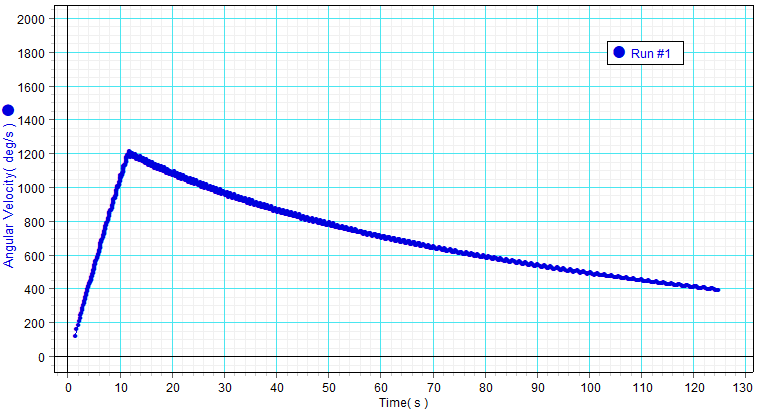
\includegraphics[scale=0.6]{velAngulard2}
\caption{Velocidade angular em função do tempo para $d=0.17\pm0.05 m $. \label{figura:5.2}}
\end{figure}

\begin{figure} [H]
\center
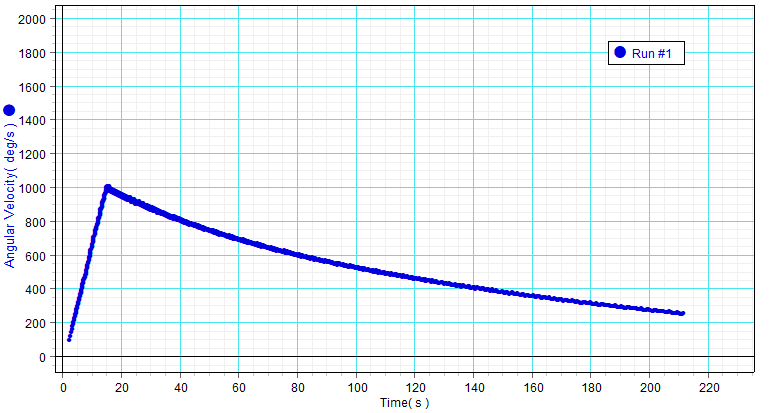
\includegraphics[scale=0.6]{velAngulard3}
\caption{Velocidade angular em função do tempo para $d=0.22\pm0.05 m $. \label{figura:5.3}}
\end{figure}

\begin{figure} [H]
\center
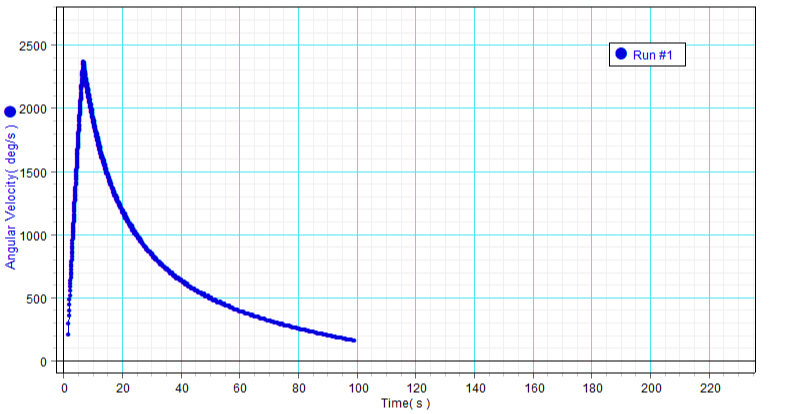
\includegraphics[scale=0.6]{velAngularSM}
\caption{Velocidade angular em função do tempo para barra sem massas cilíndricas. \label{figura:5.4}}
\end{figure}

\begin{figure} [H]
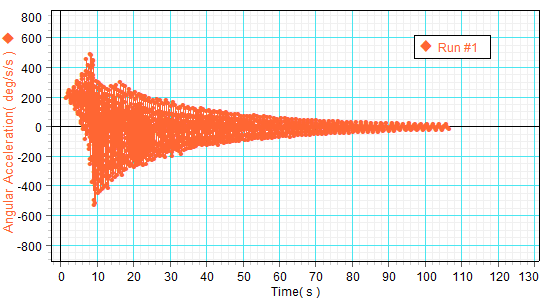
\includegraphics[scale=0.8]{angularAccelerationd1}
\caption{Aceleração angular em função do tempo para $d=0.12\pm0.05 m $. \label{figura:5.5}}
\end{figure}

\begin{figure} [H]
\center
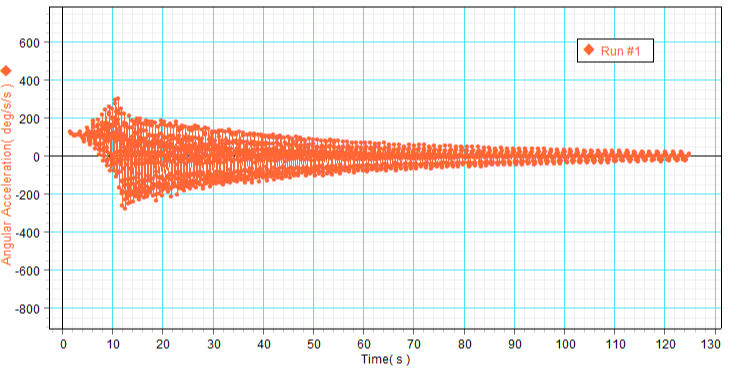
\includegraphics[scale=0.6]{angularAccelerationd2}
\caption{Aceleração angular em função do tempo para $d=0.17\pm0.05 m $. \label{figura:5.6}}
\end{figure}

\begin{figure} [H]
\center
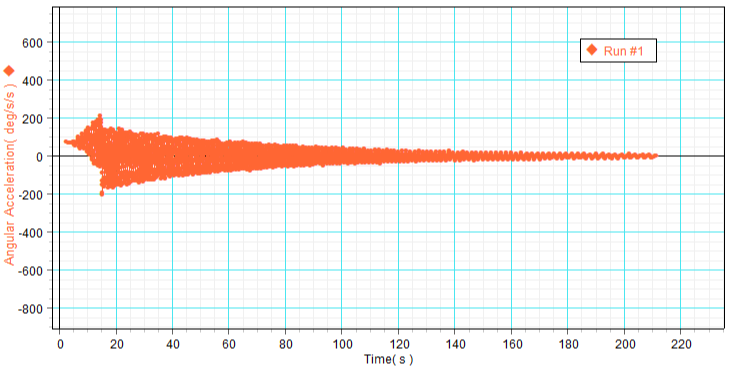
\includegraphics[scale=0.6]{angularAccelerationd3}
\caption{Aceleração angular em função do tempo para $d=0.22\pm0.05 m $. \label{figura:5.7}}
\end{figure}

\begin{figure} [H]
\center
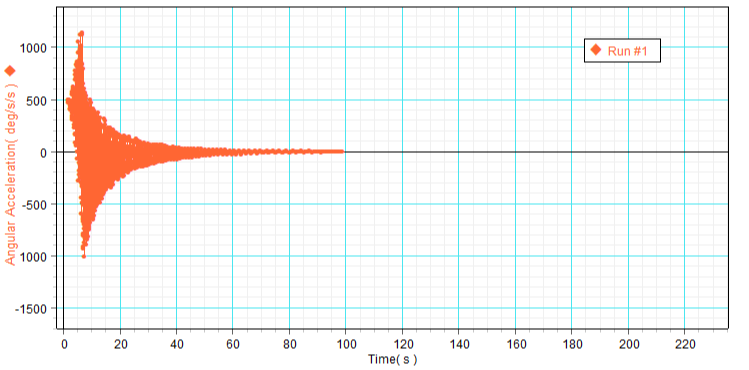
\includegraphics[scale=0.6]{angularAccelerationSM}
\caption{Aceleração angular em função do tempo para barra sem massas cilíndricas. \label{figura:5.8}}
\end{figure}


Analizando os gráficos, notamos que a velocidade angular aumenta rapidamente num primeiro instante, para todos os casos. Facilmente se conclui que tal incremento se deve à tensão do fio, que ao desenrolar pela queda da massa provoca uma aceleração angular crescente (em módulo) no sistema rotacional. Vejamos detalhadamente, por exemplo, para $d=0.12\pm0.05 m $.\\
\begin{figure} [H]
\center
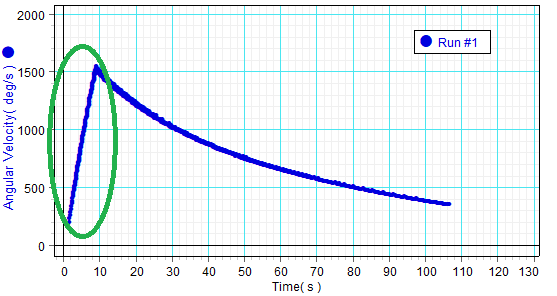
\includegraphics[scale=0.6]{velAngulard1Edited}
\caption{Velocidade angular em função do tempo para $d=0.12\pm0.05 m $, com dados referentes à queda do grave assinalados pelo anel verde. \label{figura:5.9}}
\end{figure}

\begin{figure} [H]
\center
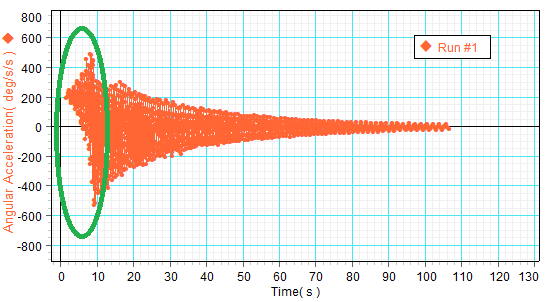
\includegraphics[scale=0.6]{angularAccelerationd1Edited}
\caption{Aceleração angular em função do tempo para $d=0.12\pm0.05 m $, com dados referentes à queda do grave assinalados pelo anel verde. \label{figura:5.10}}
\end{figure}

Nas Figuras \ref{figura:5.9} e \ref{figura:5.10} podemos ver que, na zona assinalada pelo anel verde, a velocidade angular e a aceleração angular aumentam forçosamente (em módulo). E de facto, é nestes mesmos primeiros 10 segundos que a massa está ainda ligada ao torno do sistema rotacional.\\
Podemos, então, caracterizar o movimento, até à queda da massa, como movimento acelerado. Vejamos agora o que acontece nos próximos segundos, até ao final do registo.

\begin{figure} [H]
\center
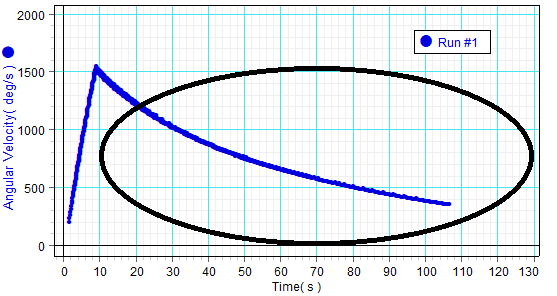
\includegraphics[scale=0.6]{velAngulard1FinalMoment}
\caption{Aceleração angular em função do tempo para $d=0.12\pm0.05 m $, com dados referentes à rotação livre de forçamento, assinalados pelo anel preto. \label{figura:5.11}}
\end{figure}

\begin{figure} [H]
\center
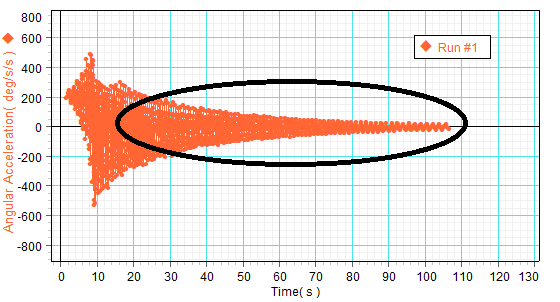
\includegraphics[scale=0.6]{angularAccelerationd1FinalMoment}
\caption{Aceleração angular em função do tempo para $d=0.12\pm0.05 m $, com dados referentes à rotação livre de forçamento, assinalados pelo anel preto. \label{figura:5.12}}
\end{figure}

Analogamente, atendendo às Figuras \ref{figura:5.11} e \ref{figura:5.12}, observamos como a velocidade angular decresce, juntamente com a aceleração angular (em módulo). Visto que o fio já se soltou e a tensão já não obriga o torno a rodar (consequentemente a barra e o disco), o sistema rotacional é deixado rodar livremente, isto se não fossem as forças de atrito presentes. \\
Podemos apontar para forças de atrito de naturezas diferentes: resistência do ar face e frição da barra ao rodar sobre o torno, entre outras. Estas forças de atrito obrigam então ao sistema a ir rodando cada vez mais devagar e, eventualmente, a parar.

Atendendo a esta divisão do movimento em duas partes\footnote{acelerado pela massa e desacelerado pelas forças de atrito}, podemos derivar as acelerações angulares associadas a cada um destes momentos. Desta forma temos
\begin{description}
\item[Para $d=0.12\pm0.05 m $]:
\begin{description}
	\item[Momento Inicial] $\alpha_i = 3.14\, rad/s^2 \pm0.45\% $
	\item[Momento Final] $\alpha_f = -0.11\, rad/s^2\pm0.03\% $
\end{description}
\item[Para $d=0.17\pm0.05 m $]:
\begin{description}
	\item[Momento Inicial] $\alpha_i = 1.88\, rad/s^2 \pm5.6\%$
	\item[Momento Final] $\alpha_f =-0.08\, rad/s^2 \pm0.02\% $
\end{description}
\pagebreak
\item[Para $d=0.22\pm0.05 m $]:
\begin{description}
	\item[Momento Inicial] $\alpha_i = 1.21\,rad/s^2\pm0.36\%$
	\item[Momento Final] $\alpha_f = -0.04\,rad/s^2\pm1.7\% $
\end{description}
\item[Para $d=0 m $]:
\begin{description}
	\item[Momento Inicial] $\alpha_i = 7.84\,rad/s^2\pm0.04\%$
	\item[Momento Final] $\alpha_f =-0.10\,rad/s^2\pm0.04\%$
\end{description}
\end{description}

Como já vimos, no momento final, as únicas forças a ser aplicada no sistema são forças de atrito. Podemos, então, dizer que a aceleração angular no momento final em cada caso é a aceleração angular média das forças de atrito.\\
Ademais da força de tensão do fio, no momento inicial, também temos forças de atrito. Desta forma, se considerarmos que a aceleração média das forças de atrito no momento final é também a aceleração média das forças de atrito no momento inicial ficamos com $$\alpha_{tens\tilde{a}o}=\alpha_i-\alpha_f. $$
Temos, então \\
\begin{description}
\item[Para $d=0.12\pm0.05 m $]: $\alpha_{tens\tilde{a}o}= 3.25\,rad/s^2\pm0.45\%$
\item[Para $d=0.17\pm0.05 m $]: $\alpha_{tens\tilde{a}o}= 1.96\,rad/s^2\pm5.1\%$
\item[Para $d=0.22\pm0.05 m $]: $\alpha_{tens\tilde{a}o}= 1.25\,rad/s^2\pm0.35\%$
\item[Para $d=0 m $]: $\alpha_{tens\tilde{a}o}= 7.94\,rad/s^2\pm0.4\%$
\end{description}

Veja-se que a tensão exercida pelo fio no torno é de igual magnitude que a tensão exercida pelo fio na massa suspensa. Daí surge
 $$\overrightarrow{P}+\overrightarrow{T}=m\overrightarrow{a} \iff mg-T=ma \iff T=m(g-a)\iff T=m(g-\alpha r). $$
 com $r$ o raio do torno e $m$ a massa suspensa.\\
 Efetuando os cálculos para cada distância dos cilindros, $d$, obtemos
 \begin{description}
 \item[Para $d=0.12\pm0.05 m $]: $a=0.0252\,m/s^2\pm0.36\%$ e $T=2.050\,N\pm0.45\%$;
\item[Para $d=0.17\pm0.05 m $]: $a=0.0152\,m/s^2\pm4.91\%$ e $T=2.052\,N\pm 5.1\%$;
\item[Para $d=0.22\pm0.05 m $]: $a=0.0097\,m/s^2\pm0.37\%$ e $T=2.054\,N\pm0.35\%$;
\item[Para $d=0 m $]: $a=0.0615\,m/s^2\pm0.12\%$ e $T=2.042\,N\pm0.4\%$.
 \end{description}
 
 Como já vimos o momento é uma das grandezas que caracteriza o movimento rotacional. Podemos então calcular o momento aplicado pela força de tensão.\\
 Temos $$\tau_{tens\tilde{a}o} = I \alpha_{tens\tilde{a}o} \iff T\times r =  I \alpha_{tens\tilde{a}o} \iff I = \frac{\alpha_{tens\tilde{a}o}}{T\times r}. $$
 Mais uma vez, efetuamos os cálculos para cada distância dos cilindros, 
 $d$:
  \begin{description}
 \item[Para $d=0.12\pm0.05 m $]: $I= 0.0108\,kgm^2\pm0.22\%$;
\item[Para $d=0.17\pm0.05 m $]: $I=0.0177\,kgm^2\pm2.5\%$;
\item[Para $d=0.22\pm0.05 m $]: $I=0.0270\,kgm^2\pm0.2\%$;
\item[Para $d=0 m $]: $I=0.0039\,kgm^2\pm0.12\%$.
 \end{description}
 
De acordo com o \textit{Teorema dos eixos paralelos}\cite{Cruz} temos
$$ I_p=I_{CM}+md^2,$$ 
pelo que será expectável encontrar uma relação entre o momento de inércia calculado acima e a distância das massas cilíndricas ao eixo de rotação, $d$. Vejamos a Figura \ref{figura:5.13}.

\begin{figure} [H]
\center
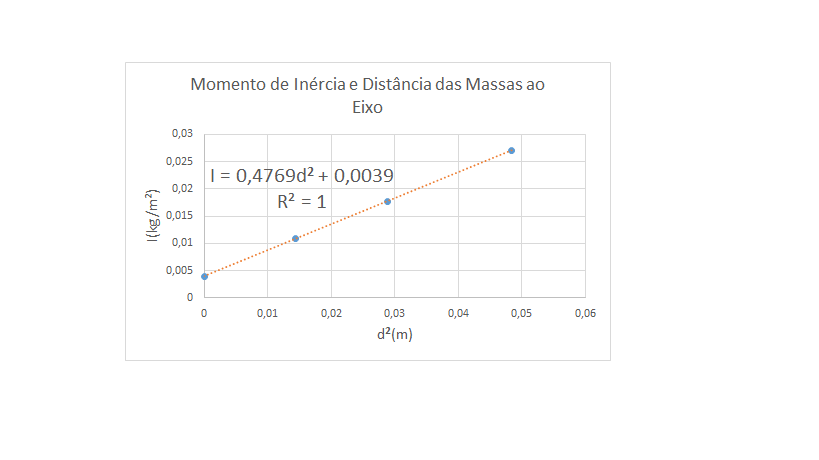
\includegraphics[scale=0.8]{inerciaEDistancia}
\caption{Relação entre a posição das massas e o momento de inércia do sistema. \label{figura:5.13}}
\end{figure}
O declive da reta da reta dá-nos a massa do corpo. Neste caso, $m=0.4769 kg.$

\chapter{Conclusão}
Finalizado o tratamento e interpretação dos dados podemos afirmar com alguma certeza que o momento de inércia de um sistema depende apenas da massa e da distribuição desta massa pelo seu volume, com ênfase na disposição da massa perpendicularmente disposta ao eixo de rotação. Durante a queda da massa concluímos, então, que há duas forças a atuar no corpo rígido: a tensão do fio ligado à massa e as forças de atrito. A força de tensão desaparece (justifique) quando o fio se solta, sobrando apenas as forças de atrito que desaceleram o corpo rígido.\\
Quanto às diferentes disposições das massas cilíndricas, podemos comentar que quanto mais afastadas estão as massas do eixo de rotação, mais tempo é requerido para parar o corpo, e sendo que no caso em que retiramos as massas, o corpo não só parou mais rápido como também atingiu uma velocidade angular máxima mais elevada que nas outras disposições.
%-------------------------------------%
%-------------BIBLIOGRAFIA------------%
\begin{thebibliography}{1}

  \bibitem{Abreu:1994} M.C. Abreu, L. Matias, L.F. Peralta {\it Física Experimental: Uma Introdução}. Editorial Presença, Lisboa: 1ª. ed., 1994. ISBN 972-23-1832-2.
  \bibitem{Serway:2014} R.A. Serway and J. W. Jewett, Jr. {\it Physics for Scientists and Engineers with Modern Physics}. Cengage, Boston: Tenth edition, 2014. ISBN 978-1-337-55329-2.
  \bibitem{Halliday:2014} Jearl Walker, David Halliday, Robert Resnick {\it Fundamentals of Physics}. Wiley, United States of America: 10th edition, 2014. ISBN 978-1-118-23072-5.
  \bibitem{Cruz} Maria Margarida Cruz {\it Dinâmica de Rotação}. Textos Complementares em Física Experimental I. Departamento de Física da Faculdade de Ciências da Universidade de Lisboa.
  \bibitem{Bulliet:2016} Richard W. Bulliet {\it 
The Wheel: Inventions and Reinventions}. Columbia University Press, United States of America: 1st Edition, 2016. ISBN 978-0-231-17338-4.



\end{thebibliography}
%-------------------------------------%
%-------------APÊNDICE----------------%
\appendix
\chapter{Figuras}
%-------------------------------------%
\begin{figure} [H]
\center
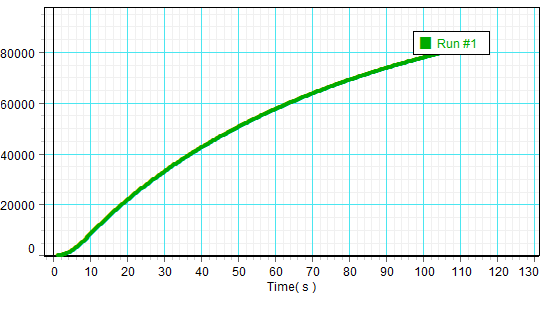
\includegraphics[scale=0.8]{angularPosition1}
\caption{Posição angular em função do tempo para $d=0.12\pm0.05 m $.}
\end{figure}

\begin{figure} [H]
\center
\includegraphics[scale=0.8]{angularPosition2}
\caption{Posição angular em função do tempo para $d=0.17\pm0.05 m $.}
\end{figure}
\begin{figure} [H]
\center
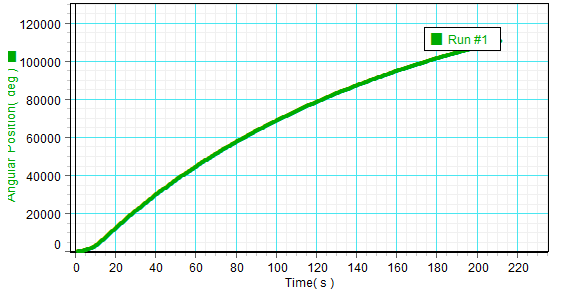
\includegraphics[scale=0.8]{angularPosition3}
\caption{Posição angular em função do tempo para $d=0.22\pm0.05 m $.}
\end{figure}
\begin{figure} [H]
\center
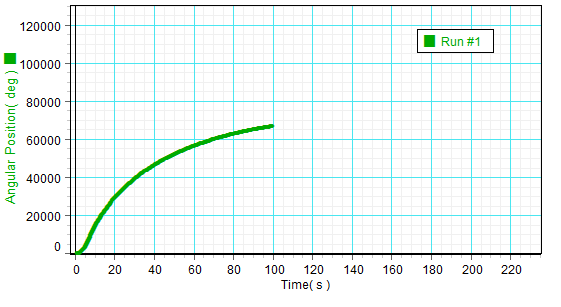
\includegraphics[scale=0.8]{angularPositionSM}
\caption{Posição angular em função do tempo para barra sem massas cilíndricas.}
\end{figure}

\begin{figure} [H]
\center
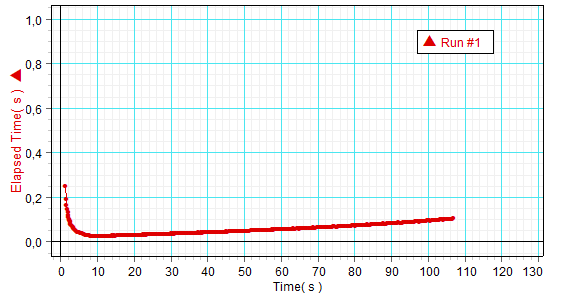
\includegraphics[scale=0.8]{elapsedTime1}
\caption{\textit{Elapsed time} para $d=0.12\pm0.05 m $.}
\end{figure}

\begin{figure} [H]
\center
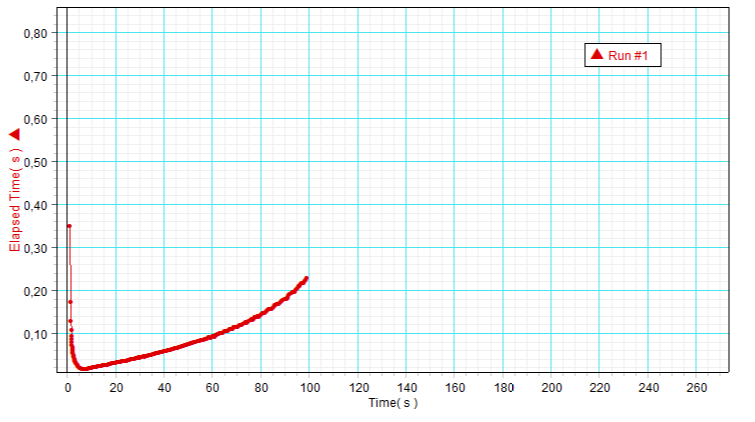
\includegraphics[scale=0.6]{elapsedTime2}
\caption{\textit{Elapsed time} para barra sem massas cilíndricas.}
\end{figure}

\end{document}